\documentclass{article}
\usepackage[top=3cm, bottom=3cm, left = 2cm, right = 2cm]{geometry}
\geometry{a4paper}
\usepackage[T1]{polski}
\usepackage[utf8]{inputenc}
\usepackage{titling}
\usepackage{caption}
\usepackage[parfill]{parskip}
\usepackage{hyperref}
\usepackage{multirow}
\usepackage{graphicx}
\usepackage{tikz}
\usetikzlibrary{decorations.markings}
\usepackage{subcaption}
\usepackage{pgffor}

\renewcommand\maketitlehooka{\null\mbox{}\vfill}
\renewcommand\maketitlehookd{\vfill\null}

\begin{document}

\begin{titlingpage}
    \title{Algorytmy metaheurystyczne\\[1ex] \large Problem komiwojażera euklidesowego. Local Search.}
    \author{Karol Janic}
    \date{16 listopada 2023}

    \maketitle
\end{titlingpage}

\tableofcontents

\newpage

\section{Cel zadania}
Celem zadania jest sprawdzenie skuteczności heurystyki Local Search na przykładzie euklidesowego problemu komiwojażera oraz
zbadanie wpływu wyboru rozwiązania początkowego i metody generowania otoczenia na jakość rozwiązania.

\section{Algorytm Local Search}
\subsection{Otoczenie invert}
Otoczeniem rozwiązania reprezentowanego przez permutację $\pi$ jest zbiór rozwiązań uzyskanych przy użyciu pojedynczego 
ruchu $invert(\pi, i, j)$, który zamienia kolejność wierzchołków od $i$-tego do $j$-tego.
\subsubsection{Moc otoczenia}
Można łatwo zauważyć, że:
\begin{itemize}
    \item $invert(\pi, i, i) = \pi$
    \item $invert(\pi, i, j) = invert(\pi, j, i)$
\end{itemize}
Zatem ruchy powodujące powstawanie różnych rozwiązań z rozwiązania $\pi$ można opisać zbiorem
(wierzchołki numerujemy liczbami od $1$ do $n$):
$$INV = \{invert(\pi, i, j) : 1 \leq i < j \leq n\}$$
Aby obliczyć moc zbioru $INV$ ustalamy $i$ kolejno na $1, 2, ..., (n-1)$ oraz dobieramy odpowiednie $j$, 
czyli $i < j \leq n$. Wtedy:
$$|INV| = (n-1) + (n-2) + ... + 1 = \frac{(n-1)n}{2} = \frac{n^2 - n}{2}$$
Interpretując permutację $\pi$ jako ciąg wierzchołków do odwiedzenia można zauważyć, że $invert(\pi, 1, n)$
nie wyprowadza nowego rozwiązania, ponieważ nie ma znaczenia czy odwiedzanie rozpoczniemy od pierwszego czy ostatniego wierzchołka, 
więc całe otoczenie ma rozmiar $\frac{n^2 - n}{2} - 1$.

\subsubsection{Własność ruchu invert}
Cechą ruchu typy invert jest "rozplątywanie" pętli w cyklu. Pętle takie są nieoptymalne. Można to pokazać korzystając z nierówności trójkata, 
która na przestrzeni euklidesowej zachodzi:
\[ d(A, D) \leq d(A, P) + d(D, P) \quad \quad d(B, C) \leq d(B, P) + d(P, C) \]

\[ d(A, C) + d(C, D) + d(D, B) = \] 
\[ = d(A, P) + d(P, C) + d(C, D) + d(D, P) + d(P, B) \geq \]
\[ \geq d(A, D) + d(D, C) + d(C, B) \]
\begin{figure}[h!]
    \centering
    \begin{subfigure}{0.5\textwidth}
        \centering
        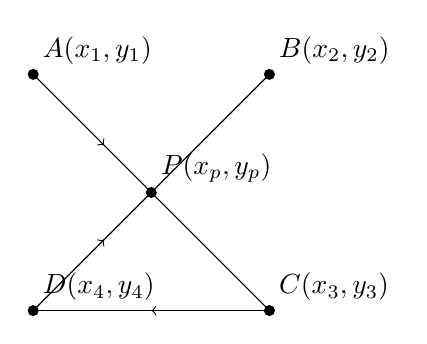
\begin{tikzpicture}
            \coordinate (A) at (0,3);
            \coordinate (B) at (3,3);
            \coordinate (C) at (3,0);
            \coordinate (D) at (0,0);
            \coordinate (P) at (1.5, 1.5);
        
            \fill (A) circle (2pt) node[above right] {$A(x_1, y_1)$};
            \fill (B) circle (2pt) node[above right] {$B(x_2, y_2)$};
            \fill (C) circle (2pt) node[above right] {$C(x_3, y_3)$};
            \fill (D) circle (2pt) node[above right] {$D(x_4, y_4)$};
            \fill (P) circle (2pt) node[above right] {$P(x_p, y_p)$};

            \draw[postaction={decorate,decoration={markings,mark=at position 0.3 with {\arrow{>}}}}] (A) -- (C);
            \draw[postaction={decorate,decoration={markings,mark=at position 0.5 with {\arrow{>}}}}] (C) -- (D);
            \draw[postaction={decorate,decoration={markings,mark=at position 0.3 with {\arrow{>}}}}] (D) -- (B);
            %\draw[postaction={decorate,decoration={markings,mark=at position 0.5 with {\arrow{>}}}}] (B) -- (A);
        
        \end{tikzpicture}
    \end{subfigure}%
    \begin{subfigure}{0.5\textwidth}
        \centering
        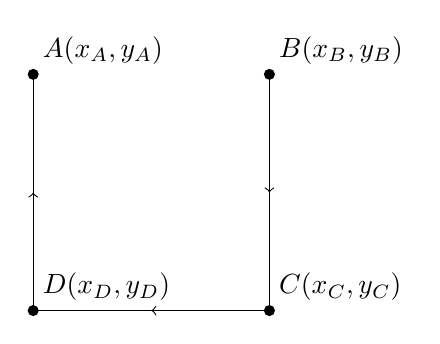
\begin{tikzpicture}
            \coordinate (A) at (0,3);
            \coordinate (B) at (3,3);
            \coordinate (C) at (3,0);
            \coordinate (D) at (0,0);
        
            \fill (A) circle (2pt) node[above right] {$A(x_A, y_A)$};
            \fill (B) circle (2pt) node[above right] {$B(x_B, y_B)$};
            \fill (C) circle (2pt) node[above right] {$C(x_C, y_C)$};
            \fill (D) circle (2pt) node[above right] {$D(x_D, y_D)$};

            %\draw[postaction={decorate,decoration={markings,mark=at position 0.5 with {\arrow{>}}}}] (A) -- (B);
            \draw[postaction={decorate,decoration={markings,mark=at position 0.5 with {\arrow{>}}}}] (B) -- (C);
            \draw[postaction={decorate,decoration={markings,mark=at position 0.5 with {\arrow{>}}}}] (C) -- (D);
            \draw[postaction={decorate,decoration={markings,mark=at position 0.5 with {\arrow{>}}}}] (D) -- (A);
            
        \end{tikzpicture}
    \end{subfigure}
\end{figure}

\newpage

\subsubsection{Problem nierówności trójkąta przy zaokrąglaniu}
W realizacji modelu odległości pomiędzy wierzchołkami wyrażane są liczbami całkowitymi. 
Konwersja dokładnej odległości następuje poprzez zaokraglenie jej do najbliższej liczby całkowitej.
W takim modelu nierówność trójkąta nie zawsze zachodzi. 
Weźmy dla przykładu powyżej punkty $A(0, 0.5)$, $B(0.5, 0.5)$, $C(0.5, 0)$, $D(0, 0)$. Wówczas punktem przecięcia jest $P(0.25, 0.25)$.
Rzeczywiste odległości prezentują się następująco: 
\[ d(A, D) = d(B, C) = 0.5 \]
\[ d(A, P) = d(D, P) = d(B, P) = d(C, P) \approx 0.35 \]
\[ d(A, C) = d(B, D) \approx 0.7 \]
Odległości w modelu prezentują się natomiast tak jak zapisano poniżej:
\[ d'(A, D) = d'(B, C) = 1 \]
\[ d'(A, P) = d'(D, P) = d'(B, P) = d'(C, P) = 0 \]
\[ d'(A, C) = d'(B, D) = 1 \]
Wtedy nierówności w $\triangle APC$ oraz $\triangle BPC$ nie zachodzą a obie skonstruowane drogi mają długość 3.

\subsection{Wybór rozwiązania początkowego}
\begin{enumerate}
    \item rozwiązanie zbudowane na podstawie MST
    \item rozwiązanie wygenerowane w sposób losowy
\end{enumerate}

\subsection{Przegląd sąsiedztwa}
\begin{enumerate}
    \item przeglądanie całego sąsiedztwa(rozmiar: $O(n^2)$)
    \item przeglądanie $n$ losowo wybranych sąsiadów(rozmiar: $O(n)$)
\end{enumerate}

\subsection{Generowanie najlepszego kandydata}
Gdy rozwiązaniem początkowym jest rozwiązanie generowane na podstawie MST to $\sqrt{n}$ razy 
generujemy takie rozwiązanie zaczynając od losowego wierzchołka drzewa a następnie 
używamy go jako startowego w algorytmie Local Search. \newline
Gdy rozwiązaniem początkowym jest rozwiązanie losowe to $n$ razy powtarzamy losowanie rozwiązania 
oraz poprawianie go algorytmem Local Search. W przypadku $n > 1000$ procedurę powtarzamy tylko 100 razy.

W każdym przypadku jako wynik wybieramy rozwiązanie o najmniejszej wadze.

\section{Wyniki}
Oznaczenia metod generujących kandydatów:
\begin{itemize}
    \item LS1 - algorytm Local Search startujący z rozwiązania wygenerowane z losowego wierzchołka MST i przeglądający całe otoczenie w każdej iteracji
    \item LS2 - algorytm Local Search startujący z losowego rozwiązania i przeglądający całe otoczenie w każdej iteracji
    \item LS3 - algorytm Local Search startujący z losowego rozwiązania i przeglądający $n$ losowych sąsiadów w każdej iteracji
\end{itemize}

Zaimplementowane metody zostały porównane na przykładach z 
\url{https://www.math.uwaterloo.ca/tsp/vlsi/index.html}. Wyniki prezentują się następująco:

\newpage

\begin{table}[h!]
    \centering
    \begin{tabular}{|c|c|c|c|c|c|}
        \hline
        \multirow{3}{*}{Przykład} & Suma wag & Suma wag & Suma wag & Suma wag  & Suma wag  \\
        & rozwiązania  & kandydata & najlepszego & najlepszego & najlepszego \\
        & optymalnego & opartego o MST & rozwiązania LS1 & rozwiązania LS2  & rozwiązania LS3 \\
        \hline
        xqf131 &  &  &  &  &  \\
        \hline
        xqg237 &  &  &  &  &  \\
        \hline
        pma343 &  &  &  &  &  \\
        \hline
        pka379 &  &  &  &  &  \\
        \hline
        bcl380 &  &  &  &  &  \\
        \hline
        pbl395 &  &  &  &  &  \\
        \hline
        pbk411 &  &  &  &  &  \\
        \hline
        pbn423 &  &  &  &  &  \\
        \hline
        pbm436 &  &  &  &  &  \\
        \hline
        xql662 &  &  &  &  &  \\
        \hline
        xit1083 &  &  &  &  &  \\
        \hline
        icw1483 &  &  &  &  &  \\
        \hline
        djc1785 &  &  &  &  &  \\
        \hline
        dcb2086 &  &  &  &  &  \\
        \hline
        pds2566 &  &  &  &  &  \\
        \hline
    \end{tabular}
    \caption{Porównanie metod generowania kandydatów dla problemu komiwojażera.}
\end{table}

\section{Wnioski}
\begin{itemize}
    \item 
\end{itemize}

% \newpage

% \section{Wizualizacje rozwiązań}
% \def \myArray{xqf131, xqg237, pma343, pka379, bcl380, pbl395, pbk411, pbn423, pbm436, xql662, xit1083, icw1483, djc1785, dcb2086, pds2566}

% \foreach \text in \myArray {
%     \subsection{\text}
    
%     \begin{figure}[h!]
%         \centering
%         \includegraphics[height=6.5cm]{../../plots/\text-tsp-mst.png}
%     \end{figure}

%     \newpage
% }

\end{document}
